% Name: Concept map
% Description: A small mind map of photosynthesis: what goes in and what comes out.
% Tags: concept map, biology, mind map

\usetikzlibrary{mindmap}

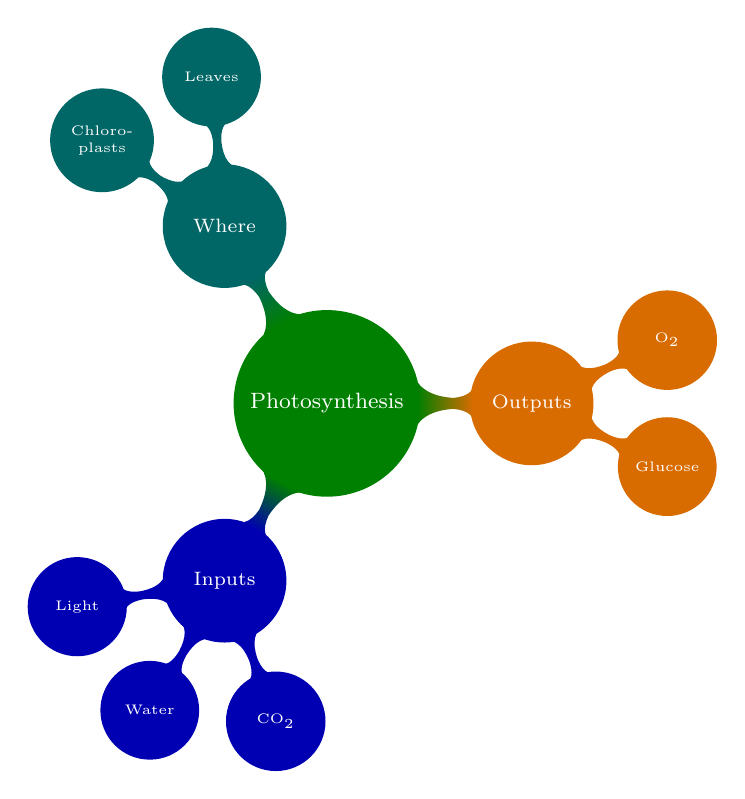
\begin{tikzpicture}[
  small mindmap, grow cyclic,
  every node/.style={concept, execute at begin node=\hskip0pt},
  concept color=green!50!black, text=white,
  level 1/.append style={level distance=2.6cm, sibling angle=120},
  level 2/.append style={level distance=1.9cm, sibling angle=50},
]
  \node {Photo\-synthesis}
    child[concept color=blue!70!black] { node {Inputs}
      child { node {Light} }
      child { node {Water} }
      child { node {CO$_2$} }
    }
    child[concept color=orange!85!black] { node {Outputs}
      child { node {Glucose} }
      child { node {O$_2$} }
    }
    child[concept color=teal!80!black] { node {Where}
      child { node {Leaves} }
      child { node {Chloro\-plasts} }
    };
\end{tikzpicture}
